% This file was created by matplotlib2tikz v0.6.18.
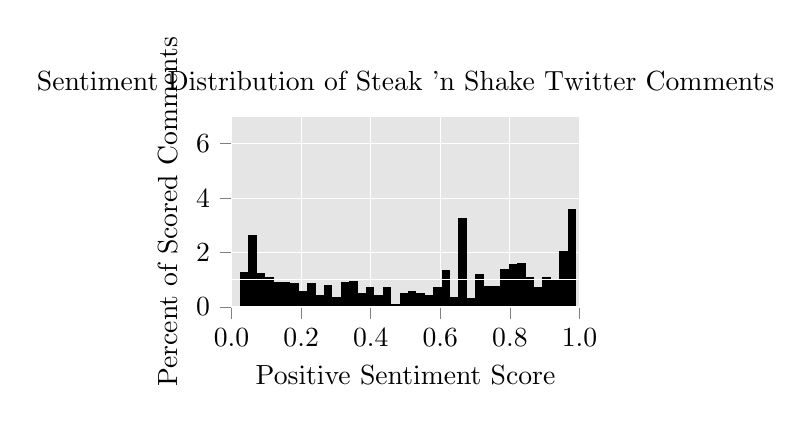
\begin{tikzpicture}

\begin{axis}[
axis background/.style={fill=white!89.80392156862746!black},
axis line style={white},
height=4cm,
tick align=outside,
tick pos=left,
title={Sentiment Distribution of Steak 'n Shake Twitter Comments},
width=6cm,
x grid style={white},
xlabel={Positive Sentiment Score},
xmajorgrids,
xmin=0, xmax=1,
xtick={0,0.2,0.4,0.6,0.8,1},
xticklabels={0.0,0.2,0.4,0.6,0.8,1.0},
y grid style={white},
ylabel={Percent of Scored Comments},
ymajorgrids,
ymin=0, ymax=7
]
\draw[fill=black,draw opacity=0] (axis cs:0.0240334682166576,0) rectangle (axis cs:0.0481831692159176,1.29401188035238);
\draw[fill=black,draw opacity=0] (axis cs:0.0481831729412079,0) rectangle (axis cs:0.0723328739404678,2.63594972002677);
\draw[fill=black,draw opacity=0] (axis cs:0.0723328739404678,0) rectangle (axis cs:0.0964825749397278,1.2460855144134);
\draw[fill=black,draw opacity=0] (axis cs:0.0964825749397278,0) rectangle (axis cs:0.120632275938988,1.10230641659647);
\draw[fill=black,draw opacity=0] (axis cs:0.120632268488407,0) rectangle (axis cs:0.144781976938248,0.91060095284056);
\draw[fill=black,draw opacity=0] (axis cs:0.144781976938248,0) rectangle (axis cs:0.168931677937508,0.91060095284056);
\draw[fill=black,draw opacity=0] (axis cs:0.168931663036346,0) rectangle (axis cs:0.193081364035606,0.862674586901583);
\draw[fill=black,draw opacity=0] (axis cs:0.193081378936768,0) rectangle (axis cs:0.217231079936028,0.575116391267722);
\draw[fill=black,draw opacity=0] (axis cs:0.217231065034866,0) rectangle (axis cs:0.241380766034126,0.862674586901583);
\draw[fill=black,draw opacity=0] (axis cs:0.241380780935287,0) rectangle (axis cs:0.265530496835709,0.431337027301634);
\draw[fill=black,draw opacity=0] (axis cs:0.265530526638031,0) rectangle (axis cs:0.28968021273613,0.814748723689413);
\draw[fill=black,draw opacity=0] (axis cs:0.289680182933807,0) rectangle (axis cs:0.313829898834229,0.383410690934786);
\draw[fill=black,draw opacity=0] (axis cs:0.313829898834229,0) rectangle (axis cs:0.337979584932327,0.910601514711697);
\draw[fill=black,draw opacity=0] (axis cs:0.337979584932327,0) rectangle (axis cs:0.362129300832748,0.958526727336965);
\draw[fill=black,draw opacity=0] (axis cs:0.362129330635071,0) rectangle (axis cs:0.38627901673317,0.527190350622561);
\draw[fill=black,draw opacity=0] (axis cs:0.386278986930847,0) rectangle (axis cs:0.410428702831268,0.718895045502724);
\draw[fill=black,draw opacity=0] (axis cs:0.410428702831268,0) rectangle (axis cs:0.434578388929367,0.431337559600278);
\draw[fill=black,draw opacity=0] (axis cs:0.434578388929367,0) rectangle (axis cs:0.458728104829788,0.718895045502724);
\draw[fill=black,draw opacity=0] (axis cs:0.458728134632111,0) rectangle (axis cs:0.482877820730209,0.0958527910222839);
\draw[fill=black,draw opacity=0] (axis cs:0.482877790927887,0) rectangle (axis cs:0.507027506828308,0.527189700035331);
\draw[fill=black,draw opacity=0] (axis cs:0.507027506828308,0) rectangle (axis cs:0.531177222728729,0.575116036402179);
\draw[fill=black,draw opacity=0] (axis cs:0.531177222728729,0) rectangle (axis cs:0.555326879024506,0.527191001211398);
\draw[fill=black,draw opacity=0] (axis cs:0.55532693862915,0) rectangle (axis cs:0.579476654529572,0.431337027301634);
\draw[fill=black,draw opacity=0] (axis cs:0.579476594924927,0) rectangle (axis cs:0.603626310825348,0.718895045502724);
\draw[fill=black,draw opacity=0] (axis cs:0.603626370429993,0) rectangle (axis cs:0.627776086330414,1.34193741827175);
\draw[fill=black,draw opacity=0] (axis cs:0.627776026725769,0) rectangle (axis cs:0.651925683021545,0.383411637244653);
\draw[fill=black,draw opacity=0] (axis cs:0.651925683021545,0) rectangle (axis cs:0.676075398921967,3.25899087294568);
\draw[fill=black,draw opacity=0] (axis cs:0.676075458526611,0) rectangle (axis cs:0.700225174427032,0.335484354567938);
\draw[fill=black,draw opacity=0] (axis cs:0.700225114822388,0) rectangle (axis cs:0.724374830722809,1.19815840917121);
\draw[fill=black,draw opacity=0] (axis cs:0.724374830722809,0) rectangle (axis cs:0.748524487018585,0.766823274489306);
\draw[fill=black,draw opacity=0] (axis cs:0.74852454662323,0) rectangle (axis cs:0.772674262523651,0.766821381869572);
\draw[fill=black,draw opacity=0] (axis cs:0.772674202919006,0) rectangle (axis cs:0.796823918819427,1.3898637546386);
\draw[fill=black,draw opacity=0] (axis cs:0.796823978424072,0) rectangle (axis cs:0.820973694324493,1.58156910010599);
\draw[fill=black,draw opacity=0] (axis cs:0.820973634719849,0) rectangle (axis cs:0.845123291015625,1.62949945828978);
\draw[fill=black,draw opacity=0] (axis cs:0.845123291015625,0) rectangle (axis cs:0.869273006916046,1.10230573643751);
\draw[fill=black,draw opacity=0] (axis cs:0.869273066520691,0) rectangle (axis cs:0.893422782421112,0.718895045502724);
\draw[fill=black,draw opacity=0] (axis cs:0.893422722816467,0) rectangle (axis cs:0.917572438716888,1.10230573643751);
\draw[fill=black,draw opacity=0] (axis cs:0.917572438716888,0) rectangle (axis cs:0.941722095012665,1.00645554776721);
\draw[fill=black,draw opacity=0] (axis cs:0.94172215461731,0) rectangle (axis cs:0.965871870517731,2.06083246377448);
\draw[fill=black,draw opacity=0] (axis cs:0.965871810913086,0) rectangle (axis cs:0.990021526813507,3.59447522751362);
\path [draw=white, fill opacity=0] (axis cs:0,0)
--(axis cs:0,7);

\path [draw=white, fill opacity=0] (axis cs:1,0)
--(axis cs:1,7);

\path [draw=white, fill opacity=0] (axis cs:0,0)
--(axis cs:1,0);

\path [draw=white, fill opacity=0] (axis cs:0,1)
--(axis cs:1,1);

\end{axis}

\end{tikzpicture}